\documentclass{article}
\usepackage{multiGWAS-preamble}

\begin{document}

\title{MultiGWAS: A tool for GWAS analysis on tetraploid organisms by integrating the results of four GWAS software}
%%Mi propuesta de título sería:
%MultiGWAS: A tool for GWAS analysis on tetraploid organisms by integrating four software
%%También puede ser -> MultiGWAS: A tool for GWAS analysis on tetraploid organisms by integrating the results of four software
%Atte: Ivania

\author[1]{L. Garreta}
\author[1]{I. Cer\'{o}n-Souza}
\author[2]{M.R. Palacio}
\author[1]{P.H. Reyes-Herrera}

\affil[1]{Corporaci\'{o}n Colombiana de Investigaci\'{o}n Agropecuaria (AGROSAVIA), CI Tibaitat\'{a},  Kil\'{o}metro 14, V\'{i}a a Mosquera, 250047, Colombia}

\affil[2]{Corporaci\'{o}n Colombiana de Investigaci\'{o}n Agropecuaria (AGROSAVIA), CI El Mira, Kil\'{o}metro 38, V\'{i}a Tumaco Pasto, Colombia}


\maketitle

%%226/250
%IAquí hice unos cambios pequeños para ampliar el espectro del estudio a cualquier planta tetraploide ya que esta revista está enfocada en herramientas para estudios evolutivos de cualquier organismo. Att. Ivania
\begin{abstract}
\textbf{Summary:} The Genome-Wide Association Studies (GWAS) are essential to determine the association between genetic variants across individuals. One way to support the results is by using different tools to validate the reproducibility of the associations. Currently, software for GWAS in diploids is well-established but for polyploids species is scarce. Each GWAS software has its characteristics, which can cost time and effort to use them successfully. Here, we present MultiGWAS, a tool to do GWAS analysis in tetraploid organisms by executing in parallel and integrating the results from four existing GWAS software: two available for polyploids (GWASpoly and SHEsis) and two frequently used for diploids (PLINK and TASSEL). The tool deals with all the elements of the GWAS process in the four software, including (1) the use of different control quality filters for the genomic data, (2) the execution of two GWAS models, the full model with control for population structure and individual relatedness and the Naive model without any control. The summary report generated by MultiGWAS provides the user with tables and plots describing intuitively the significant association found by both each one and across four software, which helps users to check for false-positive or false-negative results.\\

MultiGWAS generates five summary results integrating the four tools. (1) Score tables with detailed information on the associations for each tool. (2) Venn diagrams of shared SNPs among the four tools. (3) Heatmaps of significative SNP profiles among the four tools. (4) Manhattan and QQ plots for the association found by each tool. And (5) Chord diagrams for the chromosomes vs. SNP by each tool.
%PAULA: no se si explicamos un poco mejor el output acá?
\textbf{Contact:} phreyes@agrosavia.co\\

\textbf{Keywords: GWAS, tetraploids, SNPs,XXX}

\end{abstract}
\maketitle 

\section{Introduction}

The Genome-Wide Association Study (GWAS) is used to identify which variants through the whole genome of a large number of individuals are associated with a specific trait \cite{cantor2010prioritizing, begum2012comprehensive}. This methodology started with humans and several model plants, such as rice, maize, and $Arabidopsis$ \cite{lauc2010genomics, tian2011genome, cao2011whole, korte2013advantages, han2013sequencing}. Because of the advances in the next-gen sequencing technology and the decline of the sequencing cost in recent years, there is an increase in the availability of genome sequences of different organisms at a faster rate \cite{ekblom2011applications, ellegren2014genome}. Thus, the GWAS is becoming the standard tool to understand the genetic bases of either ecological or economic phenotypic variation for both model and non-model organisms. This increment in GWAS includes complex species such as polyploids (Fig \ref{GWASpolyploids}) \cite{ekblom2011applications, santure2018wild}. 

% Figure timelines articles
\begin{figure}
\begin{center}
%\includegraphics[width=13cm]{images/GWAStimeline.png}
    
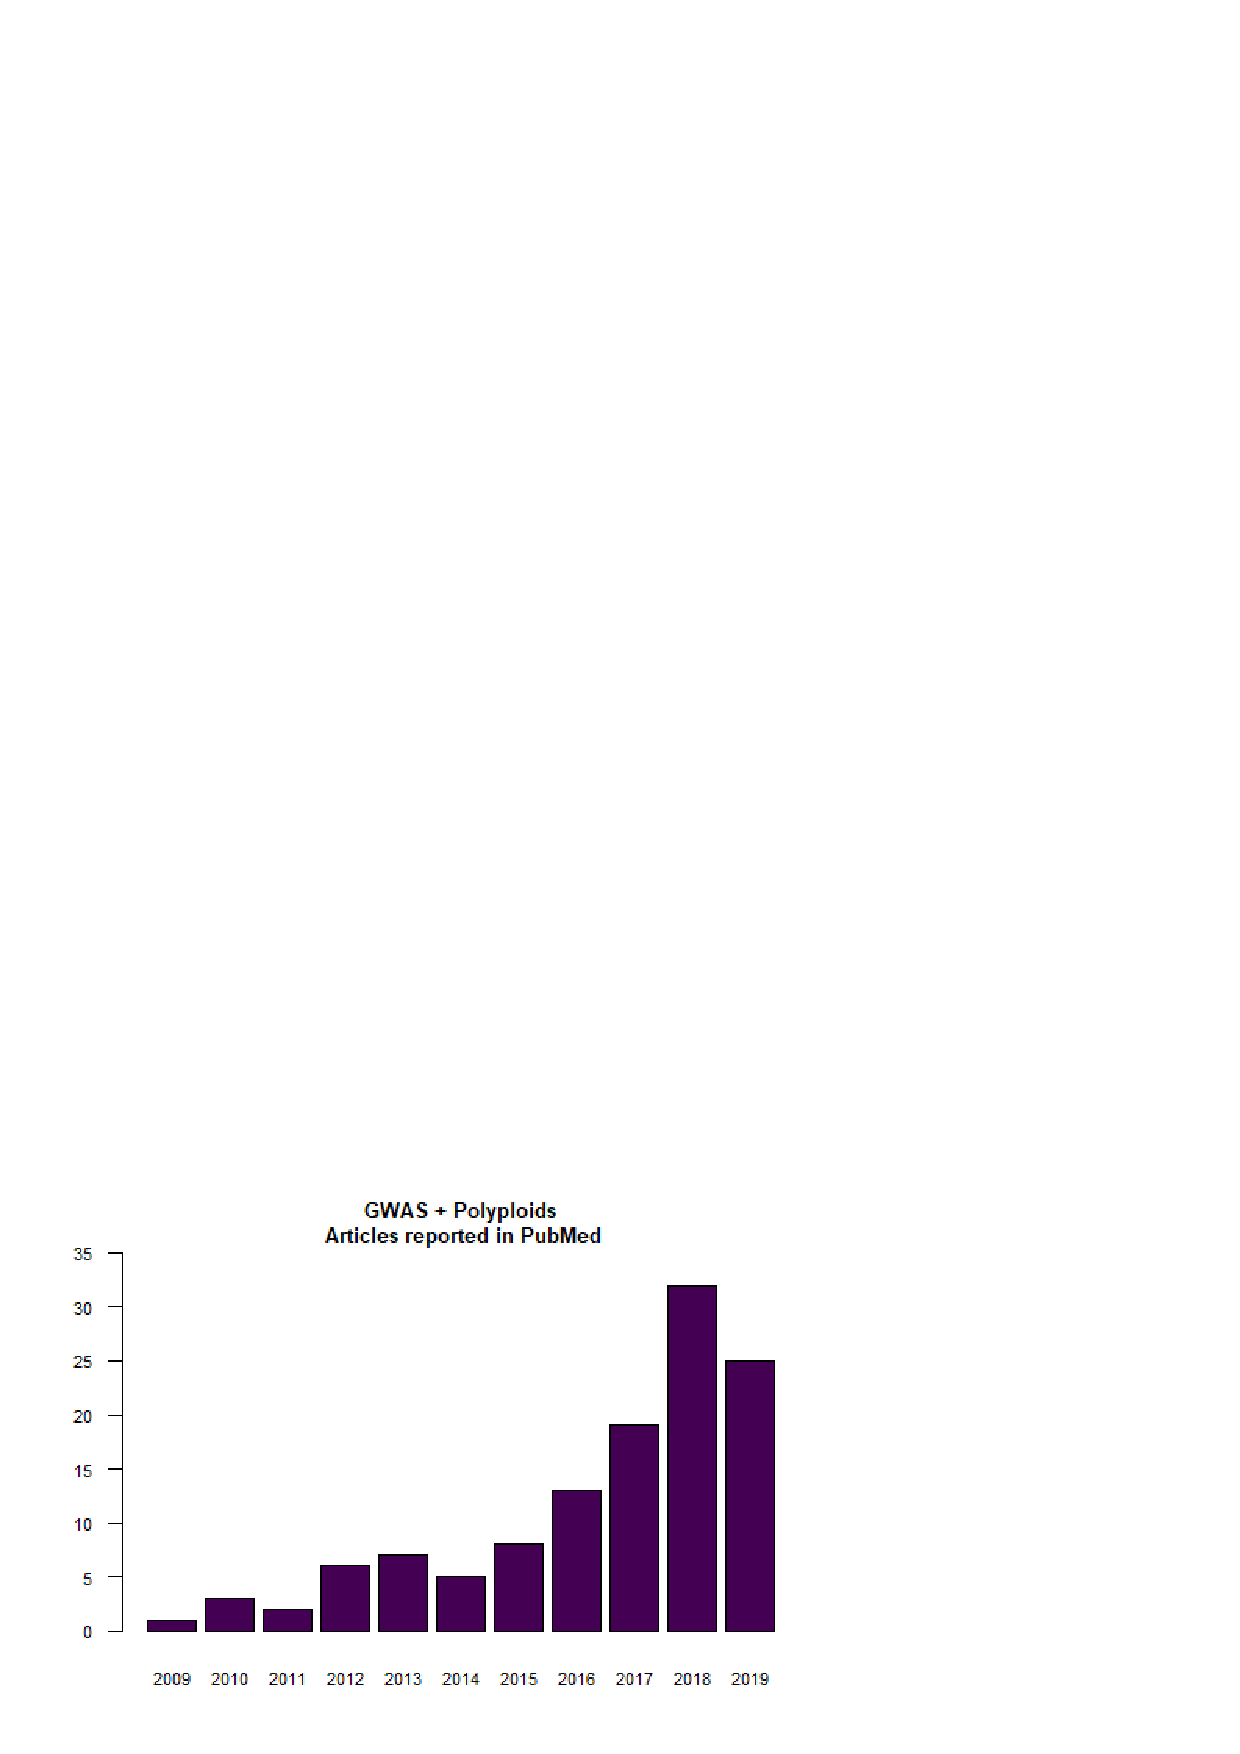
\includegraphics[width=12cm]{images/GWASpolyploids.png}

\caption{Timeline for articles reported for GWAS studies on polyploid species in PubMed. We present data for completed years.\label{GWASpolyploids}}
\end{center}

\end{figure}

The GWAS for polyploid species has three related challenges. First, as all GWAS, we should replicate the study as a reliable method to validate the results and recognize real associations. This replication involves finding the same associations either in several replicates from the study population using the same software or testing different GWAS tools among the same study population. This approach involved the use of different parameters, models, or conditions, to test how consistent the results are \cite{De2014,Pearson2008}. However, the performance of different GWAS software could affect the results. For example,  the threshold $pvalue$ for SNP significance change through four GWAS software (i.e., PLINK, TASSEL, GAPIT, and FaST-LMM) when sample size varies \cite{Yan2019}. It means that well-ranked SNPs from one package can be ranked differently in another.

Second, although there are many GWAS software available to repeat the analysis under different conditions \cite{Gumpinger2018}, most of them are designed exclusively for the diploid data matrix \cite{Bourke2018}. Therefore, it is often necessary to "diploidizing" the polyploid genomic data in order to replicate the analysis. 

Third, there are very few tools focused on the integration of several GWAS software, to make comparisons under different parameters and conditions across them. As far as we know, there is only two software with this service in mind, such as iPAT and easyGWAS. 

The iPAT allows running in a graphic interface three well-known command-line GWAS software such as GAPIT, PLINK, and FarmCPU (Chen and Zhang, 2018). However, the output from each package is separated. On the other hand, the easyGWAS allows running a GWAS analysis on the web using different algorithms. This analysis could run independently of both the computer capacity and operating system. However, it needs either several datasets available or a dataset with a large number of individuals to make replicates in order to compare among algorithms. Moreover, the output from different algorithms is separated \cite{Grimm2017}.  Thus, for both software iPAT and easyGWAS, the integrative and comparative outputs among software or algorithms are missing. 

To solve all the three challenges above, we developed the MultiGWAS tool that performs GWAS analyses for tetraploid species using four software in parallel. Our tool include GWASpoly \cite{Rosyara2016} and the SHEsis tool \cite{Shen2016} that accept polyploid genomic data, and PLINK \cite{Purcell2007} and TASSEL \cite{Bradbury2007} with the use of a "diploidized" genomic matrix. The tool deals with preprocessing data, running four GWAS tools in parallel, and create comparative reports from the output of each software to help the user to decide more intuitively the true or false associations.

\section{Method}
% Luis; modificada Mayo19 
% Ivania: Yo esto lo había modificado el viernes 15 de mayo. Hoy 20 de mayo lo vuelvo a poner tal como lo edité. 

The MultiGWAS tool has three main consecutive steps: the adjustment, the multi analysis, and the integration (Fig. \ref{fig:Pipeline}). In the adjustment step, MultiGWAS processes the configuration file. Then it cleans and filters the genotype and phenotype, and  MultiGWAS "diploidize" the genomic data. Next, during the multi analysis, each GWAS tool runs in parallel. Subsequently, in the integration step, the MultiGWAS tool scans the output files from the four packages (i.e., GWASPoly, SHEsis, PLink, and TASSEL). Finally, it generates a summary of all results that contains score tables, Venn diagrams, SNP profiles, and Manhattan plots. 


% Luis; modificada Mayo19
% Figure MultiGWAS stages
% Leyenda de la figura editada por Ivania el 20 de mayo

\subsection{Adjustment stage}

\begin{figure}
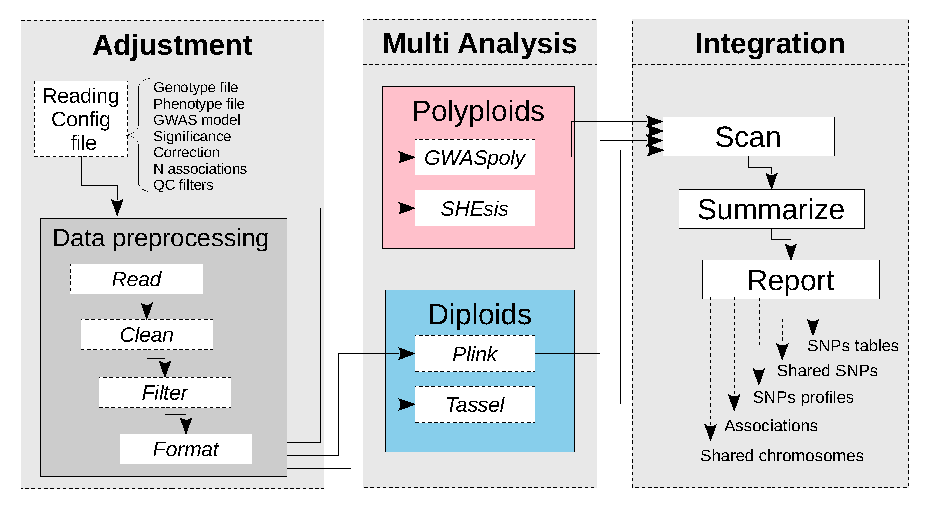
\includegraphics[width=12cm]{images/multiGWAS-flowchart-stages} \caption{MultiGWAS flowchart has three consecutive steps: adjustment, multi analysis, and integration. The adjustment step manages the input data, reads the configuration file, and preprocessing the input genomic data (genotype and phenotype). The multi analysis step configures and runs the four GWAS packages in parallel.  The integration step summarizes and reports results using different tabular and graphical visualizations.\label{fig:Pipeline}}
\end{figure}

% Luis; modificada Mayo19
% Ivania, editado mayo 20
% Me parece que esto NO ES el adjustment state sino de integration step. Yo lo cambiaria de lugar porque acá hay que describir cómo son los archivos de entrada, no los archivos de salida

%PAULA: Copiada de la 15052020 - comienzo del adjustment stage
MultiGWAS takes as input a configuration file where the user specifies the genomics data along with the parameters that will be used by the four tools. Once the configuration file is processed, MultiGWAS preprocess the data that is cleaning, filtering, and checking data quality. The output of this stage corresponds to the inputs for the four programs at the Multi Analysis stage.


\subsubsection{Reading configuration file}
The configuration file includes the following settings that we briefly describe:

\paragraph{Input genotype and phenotype files:}
Currently, MultiGWAS uses two input files, one for genotype and the other for the phenotype. Both data correspond to data matrices with column and row names (Figure \ref{fig:File-Formats}). The genotype file uses SNP markers in rows and samples in columns (Figure \ref{fig:File-Formats}a). The phenotype file uses samples in rows and traits in columns (Figure \ref{fig:File-Formats}b) with the first column corresponding to the sample name and the second column to trait value.

%Paula: Luis una pregunta, recibimos solo formato ACGT? o recibimos otro formato?? 
% R/ Actualmente solo formato GWASpoly (dos archivos), se podría facilmente formato númerido, dos archivos (ClusterCall) con o sin info de mapa (CHROM, POSITION), y tal vez formato PLINK (tres archivos).

\begin{figure}[H]
\begin{centering}
\begin{minipage}[t]{0.6\columnwidth}%
\begin{center}
\fbox{\begin{minipage}[t]{0.99\columnwidth}%
\scriptsize\texttt{Marker,Chrom,Pos,Indiv01,Indiv02,Indiv03,...}

\texttt{c2\_41437,0,805179,AAAG,AAGG,AAGG,...}

\texttt{c2\_24258,0,1252430,AAGG,AGGG,GGGG,...}

\texttt{c2\_21332,0,3499519,TTCC,TTCC,TTCC,... }

\texttt{...}%
\end{minipage}}\\
a
\par\end{center}%
\end{minipage}~~~~~~~~~%
\begin{minipage}[t]{0.3\columnwidth}%
\begin{center}
\fbox{\begin{minipage}[t]{0.99\columnwidth}%
\scriptsize\texttt{Individual,Traitname}

\texttt{Indiv01, 3.59}

\texttt{Indiv02, 4.07}

\texttt{Indiv03, 1.05}

\texttt{...}%
\end{minipage}}\\
b
\par\end{center}%
\end{minipage}
\par\end{centering}
\begin{centering}
\par\end{centering}
%Luis: ¿Qué significa "sample content o content of the sample? Me parece que eso no se entiende bien. Att. Ivania
%Editado por Ivania el 20 de mayo

\caption{\scriptsize \textbf{MultiGWAS genotype and phenotype formats}. Both files are in CSV format (Comma Separated Values) and contain as first row the header labels of the columns. Although the header labels are arbitrary, the column order is obligatory. \textbf{a.} Genotype file format, where ``Marker'', ``Chrom'', and ``Pos'', correspond to the names for marker name, chromosome, and position in the first three columns respectively. The next columns names correspond to the individual names and the column content correspond to the genotype of each individual. \textbf{b.} Phenotype file format, where ``Individual'' and ``Traitname'' are the column for the individual ID and the column for the numerical value of the trait, respectively.\label{fig:File-Formats}}
\end{figure}


%Editado por Ivania el 20 de mayo
\paragraph{GWAS model:}
MultiGWAS is designed to work with quantitative phenotypes and can run GWAS analysis using two types of statistical models that we have called \emph{full} and \emph{naive} models. The \emph{full model} is known in the literature as the Q+K model \cite{Yu2006} and includes a control for structure (Q) and relatedness between samples (K). In contrast, the \emph{naive model} does not include any correction. Both models are  
linear regression approaches, and the four GWAS packages used by MultiGWAS implemented variations of them. The \emph{naive} is modeled with Generalized Linear Models (GLMs, Phenotype + Genotype), and the \emph{full} is modeled with Mixed Linear Models (MLMs, Phenotype + Genotype + Structure + Kinship). The default model used by MultiGWAS is the \emph{full model} (Q+K) \cite{Yu2006}, following this equation:

\[
y=X\beta+S\alpha+Q\nu+Z\mu+e
\]

The vector $y$ represents the observed phenotypes depends on the following factors: the fixed effect vector $\beta$,  the SNP effects vector $\alpha$, the population effect vector $\nu$, the polygene background effect vector $\mu$, and, the residual effect vector $e$. The $Q$, modeled as a fixed effect, refers to the incidence matrix for subpopulation covariates relating $y$ to $\nu$. Moreover, $X$, $S$, and $Z$ are incidence matrices of ones and zeros relating $y$ to $\beta$, $\alpha$, and $\mu$, respectively.

%Editado por Ivania el 21 de mayo
%Luis: Solo GWASPoly y TASSEl hacen esto diferente? Si es asi se puede poner directamente que es en el caso de estos paquetes que se hace ajuste del threshold.
\paragraph{Genome-wide significance: }
GWAS searches SNPs associated with a phenotype trait in a statistically significant manner. A threshold or significance level $\alpha$ is specified and compared with the \emph{p-value} derived for each association score. Standard significance levels are 0.01 or 0.05 \cite{Gumpinger2018,Rosyara2016}, and MultiGWAS uses an $\alpha$ of 0.05 for the four GWAS packages. However, the adjustment of the threshold is according to each package. For example, GWASpoly and TASSEL calculate the SNP effect for each genotypic class using different gene action models (see ``Multi analysis stage''). Therefore, the number of tested markers\emph{ }may be different in each model (see below) that results in different \emph{p-value} thresholds.

%Editado por Ivania el 21 de mayo
\paragraph{Multiple testing correction:}
Due to the massive number of statistical tests performed by GWAS, it is necessary to perform a correction method for multiple hypothesis testing and adjusting the \emph{p-value} threshold accordingly. Two standard methods for multiple hypothesis testing are the false discovery rate (FDR) and the Bonferroni correction. The latter is the default method used by MultiGWAS because it is one of the most rigorous. MultiGWAS adjust the threshold below which a \emph{p-value} is considered significant, that is $\alpha/m$, where $\alpha$ is the significance level and \emph{m }is the number of tested markers from the genotype matrix. 

%Paula: Luis estos parametro por default de QC y alpha faltan
%Editado por Ivania el 21 de mayo
\paragraph{Number of reported associations:}
Criticism has arisen in considering only statistically significant associations as the only possible correct associations \cite{Thomson2011,Kaler2019}. Many low \emph{p-value} associations are closer to being significant, are discarded due to the stringent significance levels, and, consequently, increase the number of false negatives. To help to analyze both significant and non-significant associations, MultiGWAS provides the option to specify the number of best-ranked associations (lower \emph{p-values}), adding the corresponding \emph{p-value} to each association found. In this way, it is possible to enlarge the number of results, and we can observe replicability in the results for different programs. Nevertheless, MultiGWAS always presents each associated SNP with its corresponding \emph{p-value}.

%  We present the resultant associations in different tables and graphics reported by MultiGWAS (see Figure \ref{fig:-View-Shared-SNPs}). 
%Editado por Ivania el 21 de mayo
\paragraph{Quality control filters:}
A control step is necessary to check the input data for genotype or phenotype errors or poor quality that can lead to spurious GWAS results. MultiGWAS provides the option to select and define thresholds for the following filters that control the data quality: Minor Allele Frequency (MAF), individual missing rate (MIND), SNP missing rate (GENO), and Hardy\-Weinberg threshold (HWE):
\begin{itemize}
\item \textbf{MAF of }\textbf{\emph{x:}} filters out SNPs with minor allele frequency below \emph{x} (default 0.01); 
\item \textbf{MIND of }\textbf{\emph{x:}} filters out all individuals with missing genotypes exceeding \emph{x}{*}100\% (default 0.1); 
\item \textbf{GENO of }\textbf{\emph{x:}} filters out SNPs with missing values exceeding \emph{x}{*}100\% (default 0.1); 
\item \textbf{HWE of }\textbf{\emph{x:}} filters out SNPs which have Hardy-Weinberg equilibrium exact test \emph{p-value} below the \emph{x} threshold.
\end{itemize}
MultiGWAS does the MAF filtering and uses the PLINK package \cite{Gumpinger2018} for the other three filters: MIND, GENO, and HWE. 

%Editado por Ivania el 21 de mayo
%Luis por qué el segundo párrafo no se separa?? y además se sale del margen.
\subsubsection{Data preprocessing}
Once the configuration file is processed, the genomic data is read and cleaned by selecting individuals present in both genotype and phenotype. Then, based on previous selected quality-control filters and their thresholds, MultiGWAS remove individuals and SNPs with poor quality.

During this step, the format \textquotedbl{}ACGT\textquotedbl{} suitable for the polyploid software GWASpoly and SHEsis, is \textquotedbl{}diploidized\textquotedbl{} for PLINK and TASSEL. The homozygous tetraploid genotypes are converted to diploid thus: AAAA\textrightarrow AA, CCCC\textrightarrow CC, GGGG\textrightarrow GG, TTTT\textrightarrow TT. Moreover, for tetraploid heterozygous genotypes, the conversion depends on the reference and alternate alleles calculated for each position (e.g., AAAT\textrightarrow AT, ... ,CCCG\textrightarrow CG). 

After this process, MultiGWAS convert the genotype and phenotype data to the specific formats required for each of the four GWAS packages.

% Mayo 20: (Por Luis) Varias actualizaciones. Aparecen en color azul en el PDF
%Editado por Ivania en junio 5 de 2020
\subsection{Multi analysis stage}
MultiGWAS runs in parallel using two types of statistical models specified in the parameters file, the Full model (Q+K) and Naive (i.e., without any control) where Q refers to population structure and K refers to relatedness, calculated by kinship coeficients across individuals \cite{Sharma2018}. The Full model (Q+K) controls for both population structure and individual relatedness. For population structure, MultiGWAS uses the Principal Component Analysis (PCA) and takes the top \textcolor{blue}{five} PC as covariates. For relatedness, \textcolor{blue}{MultiGWAS} uses kinship matrices that TASSEL and GWASpoly calculated separately, and for PLINK and SHEsis, \textcolor{blue}{relatedness depends on kinship coefficients calculated with the PLINK 2.0 built-in algorithm \cite{Chang2015}. }

\subsubsection{GWASpoly}
%Editado y revisado por Ivania el 5 de junio
GWASpoly \cite{Rosyara2016} is an R package designed for GWAS in polyploid species used in several studies in plants \cite{Berdugo2017,Ferrao2018,Sharma2018,Yuan2019}. GWASpoly uses a Q+K linear mixed model with biallelic SNPs that account for population structure and relatedness. \textcolor{blue}{Also, to calculate the SNP effect for each genotypic class, GWASpoly provides eight gene action models: general, additive, simplex dominant alternative, simplex dominant reference, duplex dominant alternative,duplex dominant, diplo-general, and diplo-additive. As a consequence, the number of statistical test performed can be different in each action model and so thresholds below which the }\textcolor{blue}{\emph{p-values}}\textcolor{blue}{{} are considered significant.}

MultiGWAS is using GWASpoly version 1.3 \textcolor{blue}{with all gene action models available to find associations. The MultiGWAS reports the top }\textcolor{blue}{\emph{N }}\textcolor{blue}{best-ranked (the SNPs with lowest }\textcolor{blue}{\emph{p-values)}}\textcolor{blue}{  that the user specified in the  }\textcolor{blue}{\emph{N}}\textcolor{blue}{{}input configuration file.} The \emph{full }model used by GWASpoly includes the population structure and relatedness, which are estimated using the first five principal components and the kinship matrix, respectively, both calculated with the GWASpoly built-in algorithms.

\subsubsection{SHEsis}
%Editado por Ivania el 5 de junio
%Luis por favor revisa que el software SOLO ha sido usado en animales y humanos (que son diploides) y no hay ningún reporte en plantas. En esta afirmación hay que estar muy seguros. Att. Ivania.

SHEsis is a program based on a linear regression model that includes single-locus association analysis, among others. The software design includes polyploid species. However, their use is mainly in diploids animals and humans \cite{Qiao2015,Meng2019}.

MultiGWAS is using version 1.0, which does not take account for population structure or relatedness. Despite, MultiGWAS externally estimates relatedness for SHEsis by excluding individuals with cryptic first-degree relatedness using the algorithm implemented in PLINK 2.0 (see below).

\subsubsection{PLINK}
%Revisado y editado por Ivania el 5 de junio
PLINK is one of the most extensively used programs for GWAS in humans and any diploid species \cite{Power2016}. PLINK includes a range of analyses, including univariate GWAS using two-sample tests and linear regression models.

MultiGWAS is using two versions of PLINK: 1.9 and 2.0. Linear regression from PLINK 1.9 performs both naive and full model. For the full model, the software calculates the population structure using the first five principal components calculated with a built-in algorithm integrated into version 1.9. Moreover, version 2.0 calculates the kinship coefficients across individuals using a built-in algorithm that removes the close individuals with first-degree relatedness.

\subsubsection{TASSEL}
%Revisado y editado por Ivania el 5 de junio
TASSEL is another standard GWAS program based on the Java software developed initially for maize but currently used in several species \cite{Alvarez2017,Zhang2018}. For the association analysis, TASSEL includes the general linear model (GLM) and mixed linear model (MLM) that accounts for population structure and relatedness. \textcolor{blue}{Moreover, as GWASPoly, TASSEL provides three-gene action models to calculate the SNP effect of each genotypic class: general, additive, and dominant, and so the significance threshold depends on each action model.}

MultiGWAS is using TASSEL 5.0, \textcolor{blue}{with all gene action models used to find the }\textcolor{blue}{\emph{N }}\textcolor{blue}{best-ranked associations and reporting the top }\textcolor{blue}{\emph{N }}\textcolor{blue}{best-ranked associations (SNPs with lowest }\textcolor{blue}{\emph{p-values)}}\textcolor{blue}{.} Naive GWAS uses the GLM, and full GWAS uses the MLM with two parameters: population structure that uses the first five principal components, and relatedness that uses the kinship matrix with centered IBS method, both calculated with the TASSEL built-in algorithms. 

% Mayo 20 (Por Luis): Pequenhas adiciones y correciones.  

% Sección 2.3 Integration stage: Completada totalmente por Luis G. (Mayo 26)
%Editado por Ivania el 5 de junio
\subsection{Integration stage.}
\color{blue} The outputs resulting from the four GWAS packages are scanned and processed to identify both significant and best-ranked associations with \emph{p-values} lower than and close to a significance threshold, respectively. 

\subsubsection{Calculation of \emph{p-values }and significance thresholds}

GWAS packages compute \emph{p-value }as a measure of association between each SNP and the trait of interest. The real associations are those their \emph{p-value }drops below a predefined significance threshold. However, the four GWAS packages compute differently \emph{p-values} with the consequence to compute them too high or too low. If \emph{p-values} is too high, it would lead to false negatives or SNPs with real associations with the phenotype, but that does not reach the significance threshold. Conversely, if \emph{p-values} are too low, then it would lead to false positives or SNPs with false associations with the phenotype, but that reaches the significance threshold.

To overcome these difficulties, in the case of too high \emph{p-values}, MultiGWAS identifies and reports both significant and best-ranked associations (the ones closest to being statistically significant). Whereas, in the case of too low \emph{p-values}, MultiGWAS provides two methods for adjusting \emph{p-values} and significance threshold: the false discovery rate (FDR) that adjust \emph{p-values, }and the Bonferroni correction, that adjusts the threshold.

By default, MultiGWAS uses the Bonferroni correction that uses the significance level  $\alpha/m$ (defined by the user in the configuration file), and $m$ (the number of tested markers) to adjust the significance threshold in the GWAS study. However, the significance threshold can be different for each GWAS package as some of them use several action models to calculate the SNP effect of each genotypic class. For both PLINK and SHEsis packages, which use only one model, $m$ is equal to the total number of SNPs. However, for both GWASpoly and TASSEL packages, which use eight and three gene action models, respectively, $m$ is equal to the number of tests performed in each model, which is different between models. 

\subsubsection{Selection of significant and best-ranked associations}
After corrections, significant associations are selected as the ones with \emph{p-values} falling below a significant threshold on each GWAS package. Nevertheless, as described above, it is equally important to know the best-ranked associations closer to being statistically significant, as they may represent associations to consider for posterior analysis. 

In the case of GWAS packages with only one gene action model (PLINK and SHESIS), the best-ranked associations are the top \emph{N} identified by the package. However, in GWAS packages with several gene action models (GWASpoly and TASSEL), the best-ranked associations are selected as the top \emph{N} from the ``best action model'', the one with more shared SNP associations. In other words, from the associations identified in more than one model. \color{black}
%Luis, actualizar este párrafo!!! att. Ivania.


\subsubsection{Integration of results}
%Sección revisada y editada por Ivania el 5 de junio
% Figure several reports
\begin{figure}
\includegraphics[width=11cm]{images/report-methodologies-all-plots} \caption{\textbf{\textcolor{blue}{Reports presented by MultiGWAS}}\textcolor{blue}{.} For each tool, first a QQ plot that \textcolor{blue}{assesses} the resultant p-values. Second, a Manhattan plot for each tool with two lines, blue and red, respectively, is the lower limit for the best ranked and significative SNPs. We present two Venn diagrams, one for the significative SNPs and one for N best-ranked SNPs of each tool. We show the results for GWAspoly, PLINK, TASSEL, and SHEsis in red, green, yellow, and blue. For each SNP that is in the intersection, thus, that is predicted by more than one tool, we provide an SNP profile. \textcolor{blue}{SNPs by chromosome chord diagrams show that the strongest associations are limited to few chromosomes. Furthermore, we present tabular summaries with details of significant and best-ranked associations. }\label{fig:Reports} }
\end{figure}
At this stage, \textcolor{blue}{MultiGWAS integrates} the results to evaluate reproducible results among tools (Fig \ref{fig:Reports}). However, it still reports a summary of the results of each tool: 
\begin{itemize}
\item A Quantile-Quantile (QQ) plots for the resultant \emph{p-values} of each tool and the corresponding \textcolor{blue}{inflation factor} $\lambda$ to assess the degree of the test statistic inflation. 
\item A Manhattan plot of each tool with two lower thresholds, one for the best-ranked SNPs, and another for the significant SNPs. 
\end{itemize}
To present the replicability, we use two sets: (1) the set of all the significative SNPs provided by each tool and (2) the set of all the best-ranked SNPs. For each set, we present a Venn diagram that shows SNPs predicted exclusively by one tool and intersections that help to identify the SNPs predicted by one, two, three, or all the tools. Also, we provide detailed tables for the two sets.

For each SNP \textcolor{blue}{identified} more than once, we provide what we call the SNP profile. That is a heat diagram for a specific SNP, where each column is a genotype state AAAA, AAAB, AABB, ABBB, \textcolor{blue}{and} BBBB. Moreover, each row corresponds to a sample. Samples with close genotypes form together clusters. Thus to generate the clusters, we do not use the phenotype information. However, we present the phenotype information in the figure as the color. This figure visually provides information regarding genotype and phenotype information simultaneously for the whole population. We present colors as tones between white and black for color blind people.

MultiGWAS generates a report, one document with the content previously described. Besides, there is a folder with the individual figures just in case the user needs one. In the supplementary information, we include a report and a description of the report content\textcolor{red}{{} (supplementary information XXX)}

%PAula: infomraciOn suplementary con reporte completo y figuras. Y explicaciOn del reporte

In the following section, we present the results applied to a public dataset. 

% LuisG: Junio 02: Modificado todas las secciones 
\section{Results}

Most of the GWAS packages used by MultiGWAS are based on a linear
regression approaches, but they often produce dissimilar association
results for the same input. For example, computed \emph{p-values }for
the same set of SNPs are different between packages; SNPs with significant
\emph{p-values} for one package may be not significant for the others;
or well-ranked SNPs in one package may be ranked differently in another. 

To alleviate these difficulties, MultiGWAS produces five types of
outputs using different graphics and tabular views, these outputs
are intended to help users to compare, select, and interpret the set
of possible SNPs associated with a trait of interest. The outputs
include: 
\begin{itemize}
\item Manhattan and Q-Q plots to show GWAS associations. 
\item Venn diagrams to show associations identified by single or several
tools.
\item Heat diagrams to show the genotypic structure of shared SNPs.
\item Chord diagrams to show shared SNPs by chromosomes.
\item Score tables to show detailed information of associations for both
summary results from MultiGWAS and particular results from each GWAS
package
\end{itemize}
As an example of the functionality of the tool, here we show the outputs
reported by MultiGWAS in the tetraploid potato diversity panel, genotyped
and phenotyped as part of the USDA-NIFA Solanaceae Coordinated Agricultural
Project (SolCAP) \cite{Hirsch2013}. The complete report from MultiGWAS
for the naive and full model is in the Supplementary information (\url{https://github.com/agrosavia-bioinformatics/multiGWAS}) 


\subsection{Manhattan and QQ plots for GWAS associations }

MultiGWAS uses classical Manhattan and Quantile\textendash Quantile
plots (QQ plots) to visualize the results of GWAS analysis from each
package. In both plots, SNPs are represented by dots and their \emph{p-values}
are transformed to scores as $-log_{10}(\mathB{p-values})$ (see Figure
\ref{fig:view-qqmanhattan}). The Manhattan plot displays the SNP
association strength (y-axis) distributed in their genomic location
(x-axis), so the higher the score the stronger the association. Whereas
the QQ plot is used to visually compare the expected distribution
of \emph{p-values }(y-axis) vs. the observed distribution (x-axis),
so under the null hypothesis of no association of SNPs with the phenotype,
both distributions should coincide, and most SNPs should lie on a
diagonal line.

MultiGWAS adds special marks to the Manhattan and QQ plots to help
identify different types of SNPs: (a) In Manhattan plots, significant
SNPs are above a red line, best-ranked SNPs are above a blue line,
and shared SNPs (See Figure \ref{fig:Table-Shared-SNPs}.b) are colored
in green (b) In QQ plots, a red diagonal line indicates the expectation,
so potential associations can be observed when the number of SNPs
deviating from the diagonal is small, as in the case of monogenic
traits, or when this number is somewhat higher, as in the case of
truly polygenic traits. However, deviations for a high number of SNPs
could reflect inflated \emph{p-values }owing to population structure
or cryptic relatedness.

\begin{figure}[H]
\noindent %
\noindent\begin{minipage}[t]{1\columnwidth}%
\begin{center}
\includegraphics{images/paper-manhattan-QQ-plots}
\par\end{center}%
\end{minipage}

\caption{\textbf{MultiGWAS visualization of associations.} MultiGWAS creates
Manhattan and QQ plots for GWAS results of each GWAS packages. Here
we show the plots for one tetraploid package, GWASpoly (a), and other
diploid package, PLINK (b). \label{fig:view-qqmanhattan}}
\end{figure}


\subsection{Tables and Venn diagrams for single and shared SNPs}

MultiGWAS provides tabular and graphic views to report in an integrated
way both the best-ranked and significant SNPs identified by the four
GWAS packages (see Figure \ref{fig:Table-Shared-SNPs}). Both \emph{p-values}
and significance levels have been scaled as $-log_{10}(\mathB{p-value})$
to give high scores to the best statistically evaluated SNPs.

First, best-ranked SNPs correspond to the top-scored \emph{N} SNPs,
wheter they were assesed significant or not by its package, and with\emph{
N} defined by the user in the configuration file. These SNPs are shown
both in a SNPs table (Figure \ref{fig:Table-Shared-SNPs}.a) and in
a Venn diagram (Figure \ref{fig:Table-Shared-SNPs}.b). The table
lists them by package and sorts by decreasing score, whereas the Venn
diagram shows them emphasizing if they were best-ranked either in
a single package or in several at once (shared). And second, the significant
SNPs correspond to the ones assesed statistically significant by each
package, they are shown in a Venn diagram (Figure \ref{fig:Table-Shared-SNPs}.c),
and they are also shown in the SNPs table, marked with significance
TRUE (T) in the table of the Figure\ref{fig:Table-Shared-SNPs}.a.

\begin{figure}[H]
\begin{centering}
\includegraphics{images/paper-table-venn-best}
\par\end{centering}
\caption{\textbf{Shared SNPs Views. }Tabular and graphical views of SNP associations
identified by one or more GWAS packages (shared SNPs). SNPs identified
by all packages are marker with red background in all figures \textbf{(a)}
Table with details of the N=9 best-ranked SNPs from each GWAS package.
Each row corresponds to a single SNP and the 9 columns are: tool name,
model used by the tool, genomic control factor (inflation factor),
SNP name, chromosome, position in the genome, \emph{p-value}, score
as $-log_{10}(\mathB{p-value})$, significance threshold as $-log_{10}(\alpha/m)$
where $\alpha$ is the significance level and $m$ is the number of
tested markers, and significance as true (T) or false (F) whether
score > threshold or not. \textbf{(b)} Venn diagram of the N=9 best-ranked
SNPs. SNPs identified by all packages are located in the central intersection.
Other SNPs identified by more than one packages are located in both
upper central and lower central intersections. \textbf{(c)} Venn diagram
of the significant SNPs (score > threshold). \label{fig:Table-Shared-SNPs}}
\end{figure}

 

\subsection{Heat diagrams for structure of shared SNPs}

MultiGWAS creates a two-dimensional representation, called SNP profile,
to visualize each trait by individuals and genotypes as rows and columns,
respectively (Figure \ref{fig:SNP-profiles}). At the left, the individuals
are grouped in a dendrogram by their genotype. At the right, there
is the name or ID of each individual. At the bottom, the genotypes
are ordered from left to right, starting from the major to the minor
allele (i.e., AAAA, AAAB, AABB, ABBB, BBBB). At the top, there is
a description of the trait based on a histogram of frequency (top
left) and by an assigned color for each numerical phenotype value
using a grayscale (top right). Thus, each individual appears as a
colored line by its phenotype value on its genotype column. For each
column, there is a solid cyan line with the mean of each column and
a broken cyan line that indicates how far the cell deviates from the
mean.

Because each multiGWAS report shows one specific trait at a time,
the histogram and color key will remain the same for all the best-ranked
SNPs.

\begin{figure}[H]
\begin{centering}
\includegraphics{images/paper-heat-maps}
\par\end{centering}
\caption{\textbf{\scriptsize{}SNP profiles. }{\scriptsize{}SNP profiles for
two of the best-ranked significant SNPs shown in the figure \ref{fig:Table-Shared-SNPs}.b.
(a) SNP c2\_45606 best-ranked by the four packages (central intersection
of the Venn diagram Figure \ref{fig:Table-Shared-SNPs}.b) (b) SNP
c1\_8019 best-ranked by the two tetraploid packages (Figure \ref{fig:Table-Shared-SNPs}.b),
and also identified as significant by the same packages (at the bottom
of the Figure \ref{fig:Table-Shared-SNPs}.a). \label{fig:SNP-profiles}}}
\end{figure}


\subsection{Chord diagrams for SNPs by chromosome}

Generally, in a typical GWAS analysis the strongest associations are
signaled by several nearby-correlated SNPs located in the same chromosome,
as in manhattan plots, where these associations form neat peaks with
several SNPs showing the same signal. Conversely, no peaks are shown
when few SNPs correlate with a trait. 

However, when the analysis is performed by several GWAS packages,
as MultiGWAS does, it can identify correlated SNPs between packages
that show the same signal, what is presented by MultiGWAS through
chord diagrams. For exampele, the Figure \ref{fig:Chord-diagrams}.a
shows the chord diagram for the shared SNPs from the best-ranked associations
previously described in the Figure \ref{fig:Table-Shared-SNPs}.b.
It can be observed that most SNPs relate to chromosome 10 and only
one to chromosome 1, which is also observed in the manhattan plots
from each GWAS package (Figure \ref{fig:Chord-diagrams}.b).

\begin{figure}
\begin{centering}
\includegraphics{images/paper-chord-manhattans}
\par\end{centering}
\caption{\textbf{SNPs by chromosome.} The figure shows how the best-ranked
SNPs relate to chromosomes. \textbf{(a)} Chord diagram showing that
most SNPs related to chromosome 10. SNPs are at the top of the diagram,
chromosomes at the botton, and associations are represented by arrows
drawn from SNPs to their chromosomes. The more associations identified
in one chromosome, the wider the space of its sector. \textbf{(b)}
Manhattan plots from each GWAS packages showing two important locations
of associations: chromosome 1 and chromosome 10, marked with a blue
and red ellipsis, respectively. \label{fig:Chord-diagrams}}

\end{figure}

% LuisG: Junio 02: Modificado todas las secciones 
\section{Availability and Implementation}

The core of the MultiGWAS tool was developed in R and users can interact
with the tool by either a command line interface (CLI) developed in
R or a graphical user interface (GUI) developed in Java (Figure \ref{fig:MultiGWAS-interaction}).
Source code, examples, documentation and installation instructions
are available at \url{https://github.com/agrosavia-bioinformatics/multiGWAS}. 

\subsection{Input parameters}

MutiGWAS uses as the only input a simple configuration text file where
users set the values for the main parameters that drives the GWAS
process. The file can be created either using a general text editor
or using the MultiGWAS GUI application (see below). In both cases,
the file must have the structure shown in the Figure \ref{fig:Configuration-file}.a,
where parameter names and values are separated by colon, filenames
are enclosed in quotation marks, and TRUE or FALSE indicates wheter
filters are applied or not. In the second case, the user creates the
config file in a simple and straightforward way using the input parameter
view from the GUI application (see below).

\begin{figure}[H]
\begin{centering}

\includegraphics{images/paper-config-file}
\par\end{centering}
\caption{Configuration file for MultiGWAS. The input parameters include: the
output folder where results will be written, input genotype/phenotype
filenames, genome-wide significance threshold, method for multiple
testing correction, GWAS model, number of associations to be reported,
filtering with TRUE or FALSE whether to use quality control filters
or not. The filters are: minor allele frequency, individual missing
rate, SNP missing rate, and Hardy-Weinberg threshold. At the end the
tools parameter defines the GWAS packages to be used for the analysis.
\label{fig:Configuration-file}}
\end{figure}


\subsection{Using the command line interface}

The execution of the CLI tool is simple, it only needs to open a
linux console, change to the folder where the configuration file was
created, and type the name of the executable tool followed by the
filename of the configuration file, like this:

\begin{lstlisting}[language=bash,basicstyle={\small}]
multiGWAS Test01.config
\end{lstlisting}

Then, the tool starts the execution, showing information of the process
in the console window, and when it finishes the results are saved
to a new subfolder called \emph{``out-Test01}. Results include a
full html report containing the different views described in the results
section, along with the original graphics and summary tables created
by MultiGWAS and used to create the html report. Additionally, results
include the preprocessed tables of the main outputs generated by the
four GWAS packages used by MultiGWAS.

\subsection{Using the graphical user interface}

The MultiGWAS GUI can be executed by calling from a linux console
the following command:

\begin{lstlisting}[language=bash,basicstyle={\small}]
jmultiGWAS
\end{lstlisting}

After it opens, it shows a main frame with a tool bar at left and
four tabs at the top (Figure \ref{fig:MultiGWAS-interaction}). From
the tool bar, users can select the GWAS packages to use in the analysis\textendash two
for tetraploids and two for diploids\textendash , and start the analysis
with the current parameters (or with parameters from a previous configuration).
And, from the tabs, users can input the MultiGWAS parameters, and
view the process and results of the analysis.

.

\begin{figure}[H]
\begin{centering}
\includegraphics[scale=0.5]{images/paper-implementation-jmultiGWAS}
\par\end{centering}
\caption{\scriptsize\textbf{MultiGWAS GUI application}. Main view of the MultiGWAS
GUI application (``Inputs'' view) where users can create the configuration
file by setting values for input parameters. The GUI contains other
three views: ``Outputs'' view shows the logs of the running process.
``Results'' view shows a report in html format with the tabular
and graphics described in the results section. And, the ``Files''
view shows an embedded file manager pointing to the subfolder that
contains the files created by MultiGWAS and used to create the report.
\protect \\
\label{fig:MultiGWAS-interaction}}
\end{figure}


















\section{Discussion}
%PAULA: Falta discutir un tris los resultados a nivel de informaicón
%PAULA: Tools diploides vs Tools poliploides en poliploides - dosis de los alelos
%PAULA: ventaja de integrar - pvalores inflados de shesis  (Balance entre sensitividad y especificidad al integrar)
%selección del modelo adecuado para cada tool - %Paula: Para polyploides el modo de inheritance es complejo por eso una selección del tool basada en replicabilidad y el factor de inflación es una propuesta justificada
XXXXXXXXXXXXXXXXXXXXXXX
%Paula Consideraciones para polyploides que afectan multiGWAS requieren estudios
%polyploides allele frequencies (alllele copy number). A way to solve is considering that each allele in partial heterozygotes has an equal likekihood of being present in more tahn one copy
% HW polyploides autopolyploides tengo dudas si se cumple - porque la segregación es diferente


%\printbibliography

\bibliographystyle{plain}
\bibliography{multiGWAS}
% La bibliografia la coloqué toda en un archivo aparte "multiGWAS.bib" creado desde Mendeley y voy a compartirlerle un repositorio de Mendeley para que coloquen la bibliografía allá de forma más fácil y solo se exporte el archivo ("multiGWAS.bib") y se suba acá a overleaf (Yo puedo hacer eso)

\end{document}
